\documentclass[../main.tex]{subfiles}
\graphicspath{{\subfix{../img/}}}

\begin{document}

\section{Additional Figures}

\begin{figure}[!b]
    \centering
    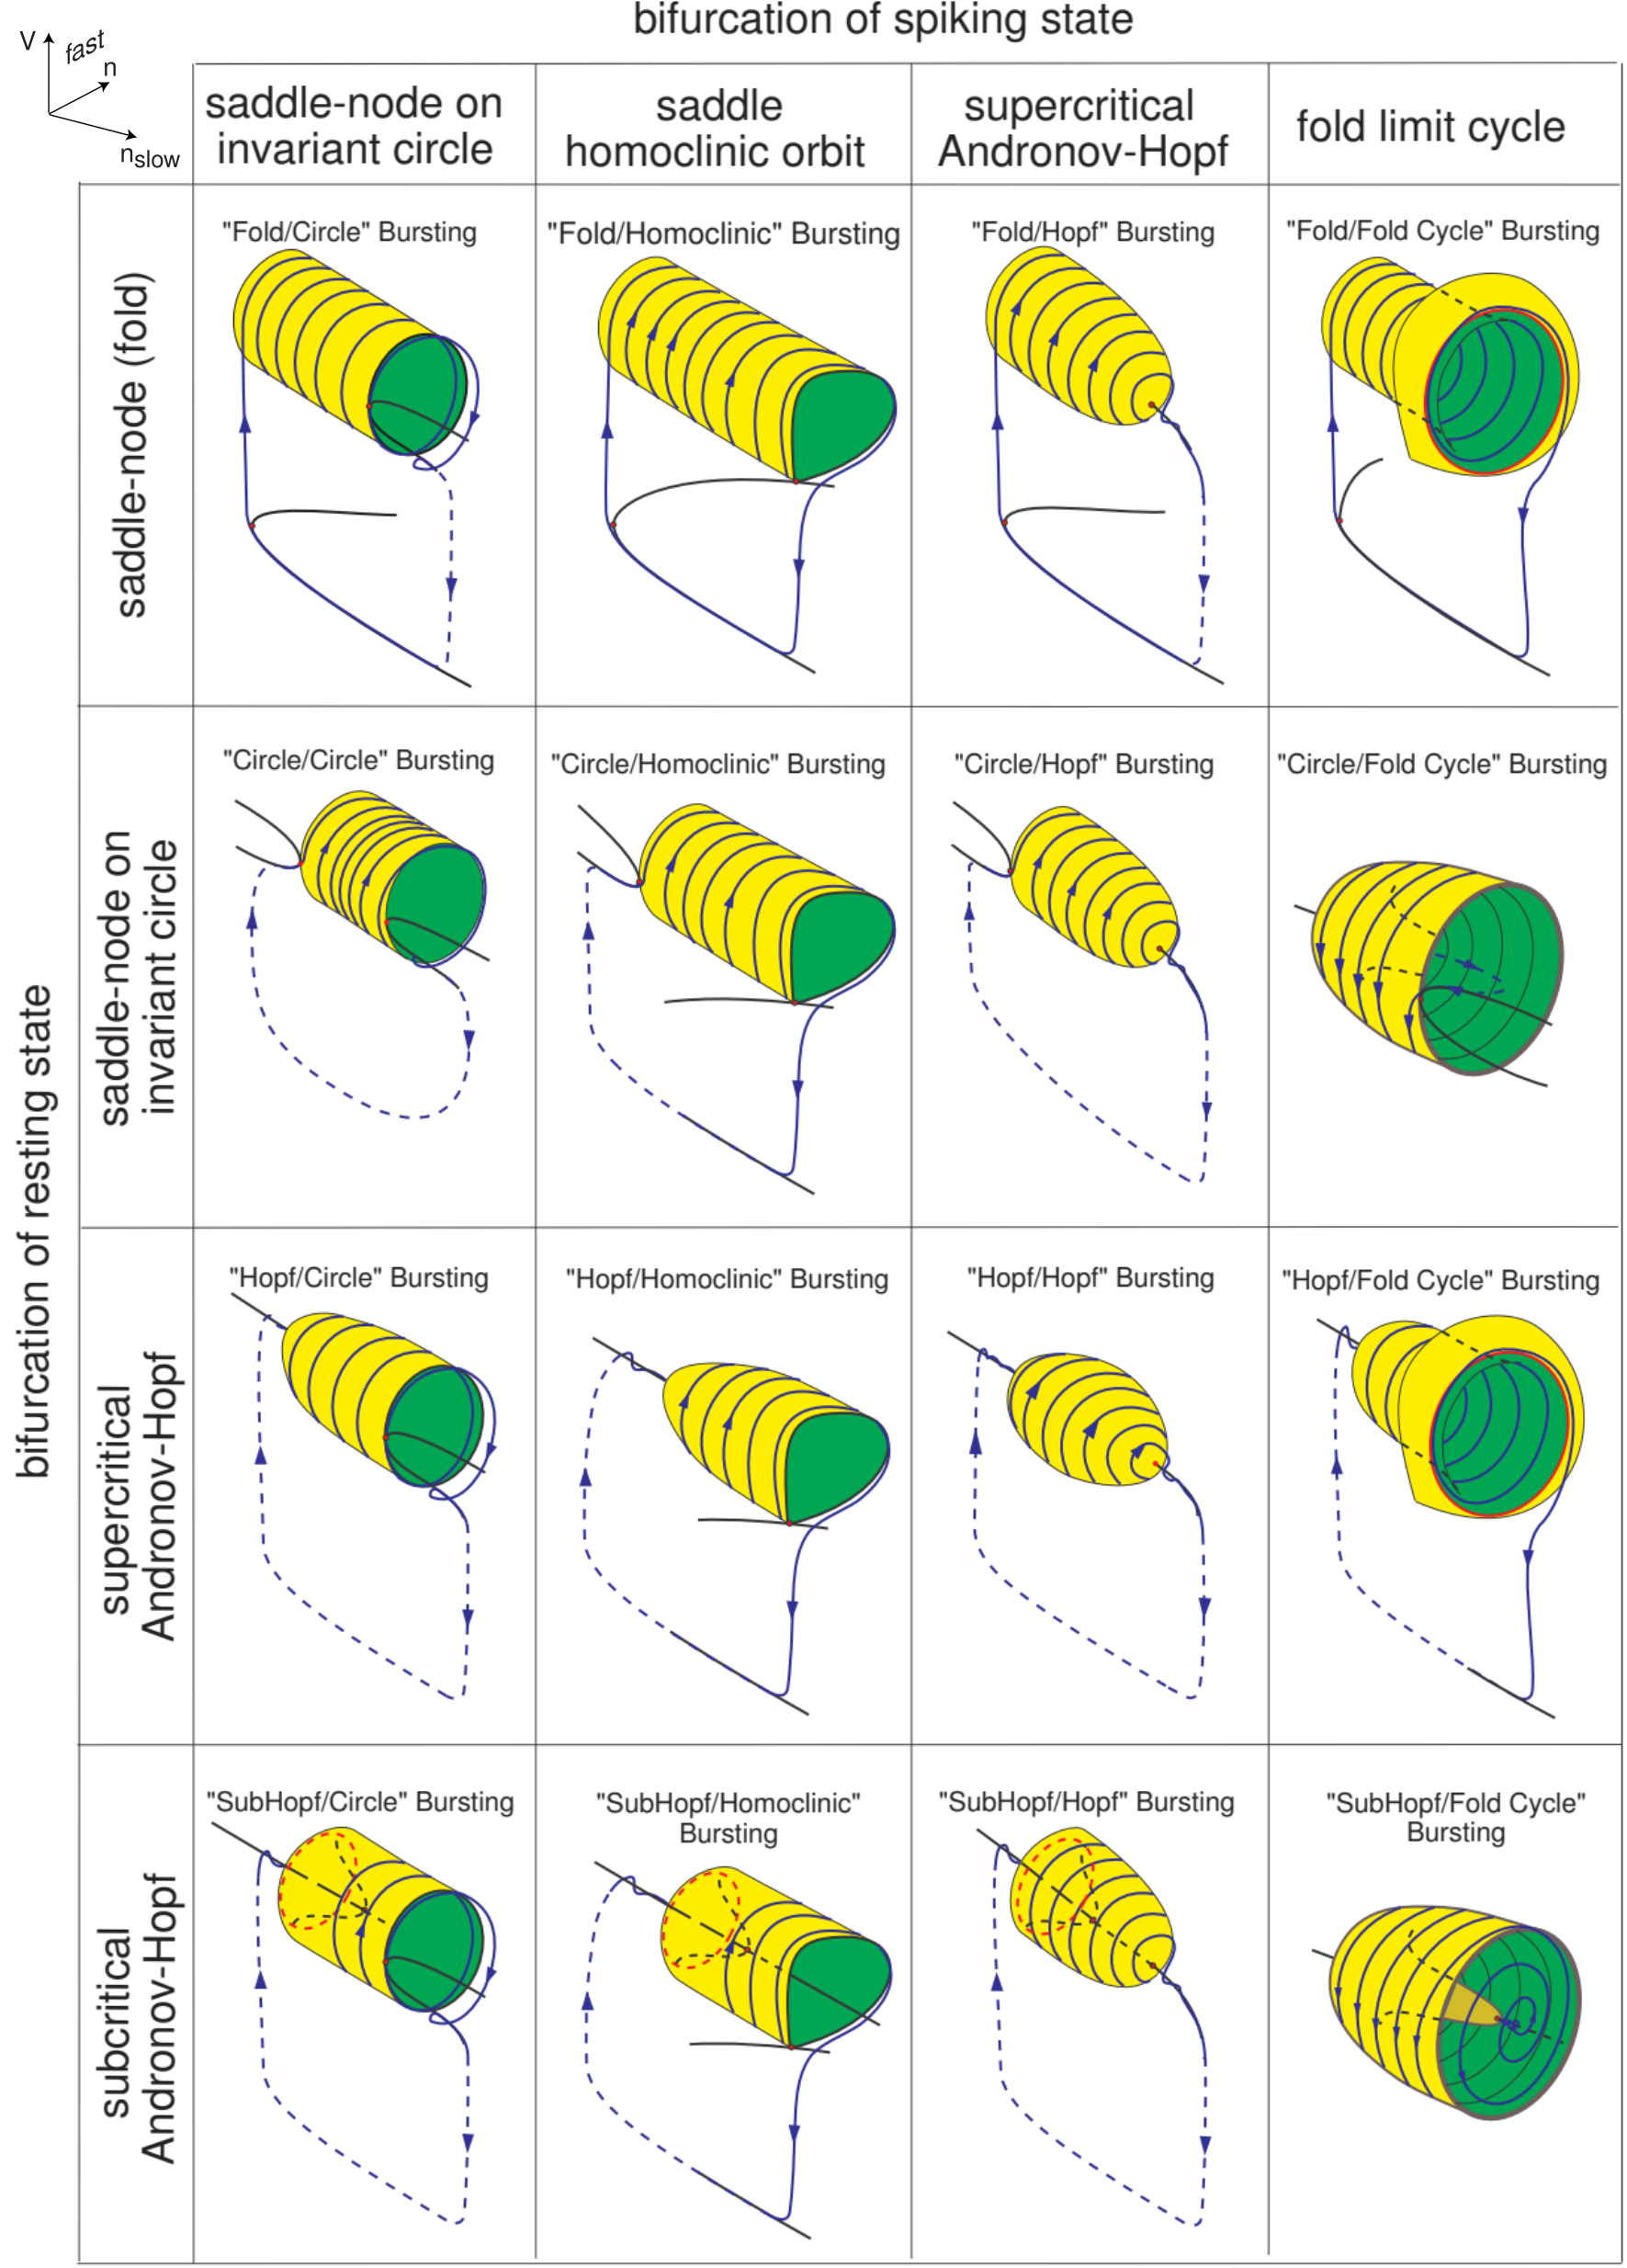
\includegraphics[width=0.75\linewidth]{../img/modelling_r5/examples/point_circle_bursters.png}
    \caption[Codimension-1 bifurcations of resting and spiking states for "2+1" point-circle bursters.]{
        Codimension-1 bifurcations of resting and spiking states for "2+1" point-circle bursters.
        The figure shows possible bifurcations for the case, when the fast (slow) system is
        two- (one-) dimensional. The inset on the top-left indicates the axis of the plots.
        $V$ - membrane potential, $n$ ($n_{slow}$) - fast (slow) variable of dynamical system.
        Adapted from \cite{izhikevichDynamicalSystemsNeuroscience2006}, with modifications.
    }
    \label{fig:izhikevich_point_circle_bursters}
\end{figure}

\end{document}